% !TeX program = lualatex
\documentclass[12pt,a4paper]{article}

% ========= حزمة =========
\usepackage[english, bidi=default, layout=counters]{babel}
\usepackage{amsmath,amssymb,amsfonts,mathtools}
\usepackage{geometry}
\geometry{left=1cm,right=1cm,top=2cm,bottom=3.1cm}   % увеличенное нижнее поле для колонтитулов
\usepackage{booktabs}
\usepackage{hyperref}
\usepackage{url}
\usepackage{graphicx}
\usepackage{caption}
\usepackage{subcaption}
\usepackage{float}
\usepackage{siunitx}
\usepackage{bm}
\usepackage{pgfplots}
\pgfplotsset{compat=1.18}
\usepackage{xcolor}
\usepackage{fontspec}
\usepackage{tikz}
\usetikzlibrary{positioning, arrows.meta, calc}
\usepackage{fancyhdr}
\usepackage{parskip}

% ========= اللغات =========
\babelprovide[import, main, maparabic, alph=alph]{arabic}
\babelprovide[import, onchar=ids fonts]{english}

% ========= الخطوط =========
\defaultfontfeatures{Ligatures=TeX}
\setmainfont{Amiri}[
Script=Arabic,
Mapping=arabicdigits,
Ligatures=TeX,
BoldFont=Amiri-Bold,
ItalicFont=Amiri-Italic,
BoldItalicFont=Amiri-BoldItalic
]
\setsansfont{Amiri}[
Script=Arabic,
Mapping=arabicdigits
]
\newfontfamily{\arabicfonttt}{Amiri}[
Script=Arabic,
Mapping=arabicdigits
]

% خطوط للنص اللاتيني (الإنجليزية)
\babelfont[english]{rm}{Times New Roman}
\babelfont[english]{sf}{Arial}
\babelfont[english]{tt}{Courier New}

% ========= ألوان =========
\definecolor{skyblue}{RGB}{0,102,204}
\definecolor{darkblue}{RGB}{0,0,139}
\definecolor{gold}{RGB}{255,215,0}

% ========= أوامر YUCT =========
\newcommand{\eps}{\varepsilon}
\newcommand{\kappac}{\kappa_c}
\newcommand{\Keff}{K_{\mathrm{eff}}}
\newcommand{\betaf}{\beta}
\newcommand{\df}{d_{\!f}}
\newcommand{\Mpl}{M_{\mathrm{Pl}}}
\newcommand{\Lpl}{l_{\mathrm{Pl}}}
\newcommand{\tP}{t_{\mathrm{P}}}
\newcommand{\Sodd}{S_{\mathrm{odd}}}
\newcommand{\Seven}{S_{\mathrm{even}}}
\newcommand{\Dtau}{\Delta\tau_{\min}}
\newcommand{\Lzero}{L_0}
\newcommand{\Omegarot}{\Omega_{\mathrm{rot}}}
\newcommand{\Mbar}{M_{\mathrm{bar}}}
\newcommand{\muniv}{M_{\mathrm{univ}}}

% ========= رؤوس وتذييلات =========
\fancypagestyle{firstpage}{%
	\fancyhf{}%
	\renewcommand{\headrulewidth}{0pt}%
	\renewcommand{\footrulewidth}{0pt}%
	\fancyfoot[C]{%
		\begin{minipage}[t]{\textwidth}
			\centering
			\textcolor{gold}{\rule{\textwidth}{1.6pt}}\\[5pt]
			{\small \textsuperscript{1}أبحاث ياكوشيف، \url{https://yuct.org/}} \hfill
			{\small بروتوكول YPSDC: \url{https://ypsdc.com/}}\\[-2pt]
			\textcolor{gold}{\rule{\textwidth}{1.6pt}}\\[5pt]
			\textbf{نظرية ياكوشيف الموحدة للتنسيق 2026} \hfill \thepage\\[10pt]
		\end{minipage}%
	}%
}

\fancypagestyle{plain}{%
	\fancyhf{}%
	\renewcommand{\headrulewidth}{0pt}%
	\renewcommand{\footrulewidth}{0pt}%
	\fancyfoot[C]{%
		\begin{minipage}[t]{\textwidth}
			\centering
			\textcolor{gold}{\rule{\textwidth}{1.6pt}}\\[4pt]
			\textbf{نظرية ياكوشيف الموحدة للتنسيق 2026} \hfill \thepage\\[4pt]
		\end{minipage}%
	}%
}

\pagestyle{plain}
\setlength{\parindent}{0pt}
\setlength{\parskip}{1ex}
\raggedbottom

\hypersetup{
	colorlinks=true,
	linkcolor=blue,
	citecolor=blue,
	urlcolor=blue,
}

% ========= رأس المقال (شعار YUCT) =========
\newcommand{\makeheader}{%
	\noindent
	\begin{minipage}{0.17\textwidth}
		\raggedright
		{\sffamily\bfseries\color{skyblue}\fontsize{46}{46}\selectfont YUCT}%
	\end{minipage}%
	\hspace{30pt}
	\begin{minipage}{0.32\textwidth}
		\raggedright
		{\sffamily\fontsize{11}{13}\selectfont نظرية ياكوشيف\\ الموحدة\\ للتنسيق}%
	\end{minipage}%
	\hfill
	\begin{minipage}{0.38\textwidth}
		\raggedleft
		{\sffamily\bfseries ملخص مكتفٍ ذاتياً}\\
		{\sffamily أبريل 2026}\\
		{\sffamily\footnotesize \url{https://doi.org/10.5281/zenodo.18444598}}%
	\end{minipage}
	\par\vspace{5pt}
	\noindent\textcolor{gold}{\rule{\textwidth}{1.6pt}}
	\par\vspace{0pt}
}

\begin{document}
	\thispagestyle{firstpage}
	\makeheader
	
	\vspace{0cm}
	{\LARGE\bfseries الكتلة الحرجة لـ YUCT والتسلسل الهرمي الكوني: ملخص مكتفٍ ذاتياً للقراء البشريين والذكاء الاصطناعي \par}
	\vspace{0.2cm}
	
	{\large أليكسي ف. ياكوشيف} \\
	\vspace{0.0cm}
	
	{\color{darkblue}\textbf{\LARGE المستخلص}} \par
	{\large
		\noindent
		تقدم هذه الوثيقة ملخصاً موجزاً ومكتفياً ذاتياً للنتائج الرئيسية من نظرية ياكوشيف الموحدة للتنسيق (YUCT) المتعلقة بالكتلة الحرجة لانفجار عظيم موضعي، ومعاملات التضخم المرتبطة به، والدوران الشامل للكون، والتسلسل الهرمي للكتلة الكونية. جميع المعادلات موسومة صراحةً كعلاقات YUCT. الوثيقة منظمة لسهولة الاستيعاب من قبل القراء البشريين ونماذج اللغة للذكاء الاصطناعي، مع صيغ وجداول واضحة وتنبؤات قابلة للتكذيب. يُعرض تسلسل هرمي كامل للكتل من مقياس بلانك إلى الكون المرصود، مما يُظهر توحيد المقاييس الكمومية والنجمية والكونية من خلال قانون قياس تنسيقي واحد.
	}
	
	\vspace{0.1cm}
	\noindent
	{\color{darkblue}\textbf{الكلمات المفتاحية:}} YUCT، الكتلة الحرجة، التضخم، الدوران الكوني، التسلسل الهرمي للكتلة، شبكة التنسيق.
	
	\vspace{0.4cm}
	
	\section{المسلمات الأساسية لـ YUCT}
	
	\begin{itemize}
		\item \textbf{كفاءة التنسيق} (بروتوكول YPSDC، الملحق B):
		\[
		\Keff = \frac{H(\mathcal{A})}{H(\kappa)}, \qquad\text{(YUCT-1)}
		\]
		حيث \(H(\mathcal{A})\) هي إنتروبيا الفعل المُنشَّط و\(H(\kappa)\) هي إنتروبيا الدليل القصير المرسَل.
		
		\item \textbf{قانون قياس الخطأ الشامل} (الملحق L):
		\[
		\varepsilon = \kappac \alpha \Keff^{-\betaf}, \qquad \betaf = \frac{2}{3},\ \kappac = \frac{1}{3}. \qquad\text{(YUCT-2)}
		\]
		
		\item \textbf{الحلقة الجبرية} (الملحق Y):
		\[
		\Sodd = \frac{6}{5},\quad \Seven = \frac{4}{5},\quad \frac{\Sodd}{\Seven} = \frac{3}{2} = \frac{1}{\betaf}. \qquad\text{(YUCT-3)}
		\]
		كمات الطول والزمن الأساسية:
		\[
		\Lzero = \frac{2}{3}\Lpl,\qquad \Dtau = \frac{2}{3}\tP. \qquad\text{(YUCT-4)}
		\]
		
		\item \textbf{البعد الكسيري} من تشبع المعلومات (الملحق L):
		\[
		d_f = \frac{11}{5}=2.2. \qquad\text{(YUCT-5)}
		\]
	\end{itemize}
	
	\section{الكتلة الحرجة لانفجار عظيم موضعي}
	
	باستخدام قانون القياس المشتق من اتساق شبكة التنسيق،
	\[
	\Keff(R) = \left(\frac{R}{\Lzero}\right)^{\betaf d_f/2}, \qquad\text{(YUCT-6)}
	\]
	وشرط الحرج \(\varepsilon \approx 1\) (أي \(\Keff = K_{\mathrm{crit}} = 3^{3/2}\))، نحصل على الكتلة الحرجة لمنطقة مرتبطة جذبياً قبل الانهيار:
	\[
	M_{\mathrm{crit}} = 3 M_{\mathrm{Pl}} \approx 6.5\times 10^{-8}\ \mathrm{kg}. \qquad\text{(YUCT-7)}
	\]
	يستخدم الاشتقاق نصف قطر شفارتزشيلد \(R_S = 2GM/c^2\) والحلقة الجبرية \(\Lzero = \frac{2}{3}\Lpl\). التصحيحات الكمومية تترك المعامل 3 دون تغيير في الرتبة الرئيسية.
	
	\section{التضخم الكوني كانقال طور تنسيقي}
	
	قابليات الرصد التضخمية مُتنبأ بها من نفس المسلمات:
	\begin{align}
		n_s &= 1 - 2\betaf^2 + \frac{4}{3}\betaf^3 + \cdots \approx 0.965, \qquad\text{(YUCT-8)}\\
		r &= 8(2\betaf)^2 = 32\betaf^2 \approx 0.07, \qquad\text{(YUCT-9)}\\
		f_{\mathrm{NL}}^{\mathrm{local}} &= \frac{5}{3}\betaf \approx 1.12. \qquad\text{(YUCT-10)}
	\end{align}
	هذه التنبؤات قابلة للتكذيب بواسطة CMB‑S4، LiteBIRD، Euclid، وSPHEREx.
	
	\section{الدوران الشامل للكون}
	
	ثنائي قطب CMB ناتج جزئياً عن دوران شامل صلب بسرعة زاوية \(\omega\). تنمو سعة ثنائي القطب مع الانزياح نحو الأحمر \(z\) كـ:
	\[
	v_{\mathrm{dip}}(z) = v_{\mathrm{local}} + \omega\, r(z). \qquad\text{(YUCT-11)}
	\]
	من النمو المرصود في NVSS وQuaia ومسوحات أخرى، نحصل على
	\[
	\omega \approx 8.5\times 10^{-22}\ \mathrm{rad/s},\qquad
	T_{\mathrm{rot}} = \frac{2\pi}{\omega} \approx 2.3\times 10^{14}\ \mathrm{yr}. \qquad\text{(YUCT-12)}
	\]
	معامل الدوران اللامُبعد هو
	\[
	\Omega_{\mathrm{rot}} \equiv \frac{\omega}{H_0} = \frac{\Seven}{\Sodd} \betaf^2 \mathcal{F}(d_f)\left(\frac{L_0}{R_H}\right)^{2\betaf} \approx 3.9\times 10^{-4}, \qquad\text{(YUCT-13)}
	\]
	ويحقق معامل هابل \(H_0 = \betaf\,\omega\). تتبع الكتلة الباريونية للكون من الدوران:
	\[
	\Mbar = \Omega_b\frac{\betaf^2 c^3}{G H_0} \approx (2.3\pm 0.2)\times 10^{51}\ \mathrm{kg}. \qquad\text{(YUCT-14)}
	\]
	
	\section{التسلسل الهرمي الكامل للكتلة من الكم إلى الكون}
	
	في YUCT، جميع الكتل من مقياس بلانك إلى الكون المرصود تخضع لقانون قياس تنسيقي واحد. يعرض الجدول~\ref{tab:full-hierarchy} مستويات التسلسل الهرمي، والكتل النموذجية، والأمثلة، وعلاقات القياس لـ YUCT المقابلة. ويوضح الشكل~\ref{fig:hierarchy-scheme} درجات السلم المتقطع.
	
	\begin{otherlanguage}{english}
		\begin{table}[htbp]
			\centering
			\caption{التسلسل الهرمي الكامل للكتلة من الكم إلى الكون (YUCT).}
			\label{tab:full-hierarchy}
			\small
			\begin{tabular}{l c c l}
				\toprule
				\textbf{Level} & \textbf{Typical mass (kg)} & \textbf{Examples} & \textbf{YUCT scaling relation} \\
				\midrule
				Planck seed & \(M_{\mathrm{crit}} = 3M_{\mathrm{Pl}} \approx 6.5\times10^{-8}\) & Local Big Bang seed & \(M_{\mathrm{crit}} = 3 M_{\mathrm{Pl}}\) (YUCT-7) \\
				Electron & \(m_e \approx 9.1\times10^{-31}\) & Lightest charged fermion & \(m_e = M_{\mathrm{Pl}} (2/3)^{96+\sigma}\xi_e\) \\
				Proton & \(m_p \approx 1.67\times10^{-27}\) & Stable baryon & \(m_p = M_{\mathrm{Pl}} (2/3)^{96+\sigma}\xi_p\) \\
				White dwarf & \(\sim 10^{30}\) (\(0.6M_\odot\)) & Chandrasekhar limit & \(M_{\mathrm{WD}} \propto M_{\mathrm{Pl}}^{3}/m_p^2\) \\
				Neutron star & \(\sim 3\times10^{30}\) (\(1.4M_\odot\)) & TOV limit & \(M_{\mathrm{NS}} \propto M_{\mathrm{Pl}}^{3}/m_p^2\) \\
				Supermassive BH & \(\sim 10^{36}\)–\(10^{40}\) & Galactic centers & \(M_{\mathrm{BH}} \propto M_{\mathrm{Pl}} (2/3)^{N}\) \\
				Observable Universe & \(M_{\mathrm{univ}} \approx 1.5\times10^{53}\) & Total mass within \(R_H\) & \(M_{\mathrm{univ}} = \frac{\betaf^2 c^3}{G H_0}\) (YUCT-14) \\
				Baryonic Universe & \(M_{\mathrm{bar}} \approx 2.3\times10^{51}\) & Visible matter & \(M_{\mathrm{bar}}/m_p = (M_{\mathrm{Pl}}/m_e)^{3.5}\) (YUCT-15) \\
				\bottomrule
			\end{tabular}
		\end{table}
	\end{otherlanguage}
	
	\begin{otherlanguage}{english}
		\begin{figure}[htbp]
			\centering
			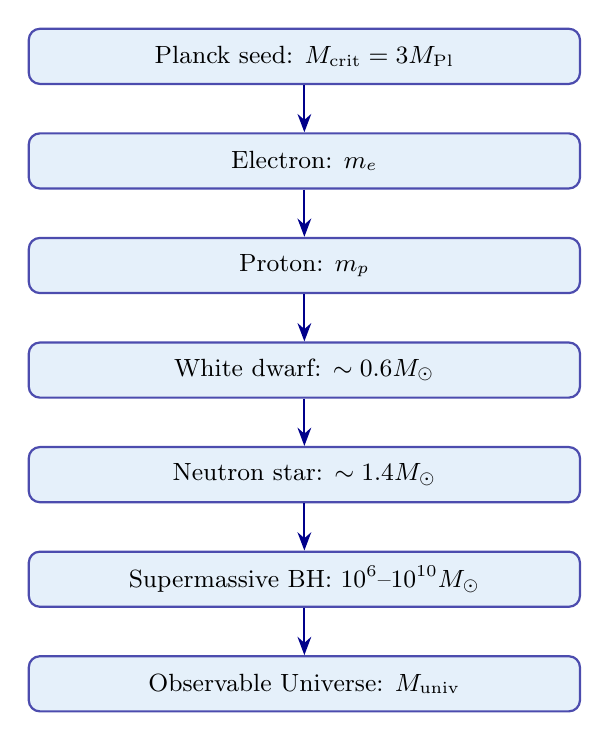
\begin{tikzpicture}[
				level/.style={rectangle, draw=darkblue!70, fill=skyblue!10, thick, minimum width=7cm, minimum height=0.7cm, rounded corners, align=center, font=\small},
				arrow/.style={->, >=Stealth, thick, color=darkblue},
				]
				\node[level] (planck) {Planck seed: \(M_{\mathrm{crit}} = 3M_{\mathrm{Pl}}\)};
				\node[level, below=0.6cm of planck] (electron) {Electron: \(m_e\)};
				\node[level, below=0.6cm of electron] (proton) {Proton: \(m_p\)};
				\node[level, below=0.6cm of proton] (wd) {White dwarf: \(\sim 0.6 M_\odot\)};
				\node[level, below=0.6cm of wd] (ns) {Neutron star: \(\sim 1.4 M_\odot\)};
				\node[level, below=0.6cm of ns] (bh) {Supermassive BH: \(10^6\)–\(10^{10} M_\odot\)};
				\node[level, below=0.6cm of bh] (univ) {Observable Universe: \(M_{\mathrm{univ}}\)};
				\draw[arrow] (planck) -- (electron);
				\draw[arrow] (electron) -- (proton);
				\draw[arrow] (proton) -- (wd);
				\draw[arrow] (wd) -- (ns);
				\draw[arrow] (ns) -- (bh);
				\draw[arrow] (bh) -- (univ);
			\end{tikzpicture}
			\caption{سلم الكتلة المتقطع من بذرة بلانك إلى الكون في YUCT. كل درجة تقابل رنيناً لحقل التنسيق.}
			\label{fig:hierarchy-scheme}
		\end{figure}
	\end{otherlanguage}
	
	يلخص التسلسل الهرمي للكتلة الكونية أيضاً بالعلاقة الجبرية
	\[
	\boxed{\frac{\Mbar}{m_p} = \left(\frac{M_{\mathrm{Pl}}}{m_e}\right)^{\mathcal{S}}},\qquad
	\mathcal{S} \equiv \Sodd + \Seven + \frac{\Sodd}{\Seven} = 3.5. \qquad\text{(YUCT-15)}
	\]
	عددياً، \((M_{\mathrm{Pl}}/m_e)^{3.5} \approx 1.88\times 10^{78}\)، وهو يتوافق مع \(\Mbar/m_p \approx 1.4\times 10^{78}\) المرصودة ضمن عامل 1.3، ويُفسر التناقض بكفاءة إعادة التسخين \(\epsilon_{\mathrm{reh}}\approx 0.85\) والعامل الهندسي \(\mathcal{F}_{\mathrm{rot}}\approx 0.9\). هذا يُظهر أن الثوابت الجبرية نفسها \(S_{\mathrm{odd}}, S_{\mathrm{even}}\) التي تحكم أُس الخطأ الشامل تحدد أيضاً الميزانية الباريونية الكونية.
	
	\section{تسلسل هرمي للأجسام الكونية والدوران الحرج}
	
	بالنسبة للأنظمة ذاتية الجذب المدعومة بضغط الانحلال، تتنبأ YUCT بقياس شامل للسرعة الزاوية الحرجة:
	\[
	\Omega_{\mathrm{crit}} \propto M^{\betaf},\qquad \betaf = 2/3. \qquad\text{(YUCT-16)}
	\]
	يوضح الجدول~\ref{tab:objects} والشكل~\ref{fig:omega-mass} هذا التسلسل الهرمي من الكواكب إلى الكون المرصود.
	
	\begin{otherlanguage}{english}
		\begin{table}[htbp]
			\centering
			\caption{المعاملات الحرجة لأجسام كونية مختارة (YUCT).}
			\label{tab:objects}
			\small
			\begin{tabular}{l c c c}
				\toprule
				\textbf{Object} & \textbf{Mass (\(M_\odot\))} & \(\log_{10}(\Omega_{\mathrm{crit}}/\mathrm{s^{-1}})\) & \textbf{Scaling law} \\
				\midrule
				Gas giant (Jupiter) & 0.001 & \(-3.8\) & \(R\sim M^{-0.67}\) \\
				Red dwarf (M5V) & 0.2 & \(-4.5\) & \(L\sim M^{2.3}\) \\
				White dwarf & 0.6 & 0.2 & \(R\sim M^{-1/3}\) \\
				Neutron star & 1.4 & 3.7 & \(M\sim\Lambda^{0.67}\) \\
				Supramassive NS & 2.2 & 4.2 & \(\Omega_{\mathrm{crit}}\sim M^{0.67}\) \\
				Stellar‑mass BH & 5 & -- & \(R_S\sim M\) \\
				Observable Universe & \(7.5\times10^{22}\) & \(-17.7\) (\(H_0\)) & \(\rho_c\sim H^2\sim K_{\mathrm{eff}}^{2/3}\) \\
				\bottomrule
			\end{tabular}
		\end{table}
	\end{otherlanguage}
	
	\begin{otherlanguage}{english}
		\begin{figure}[htbp]
			\centering
			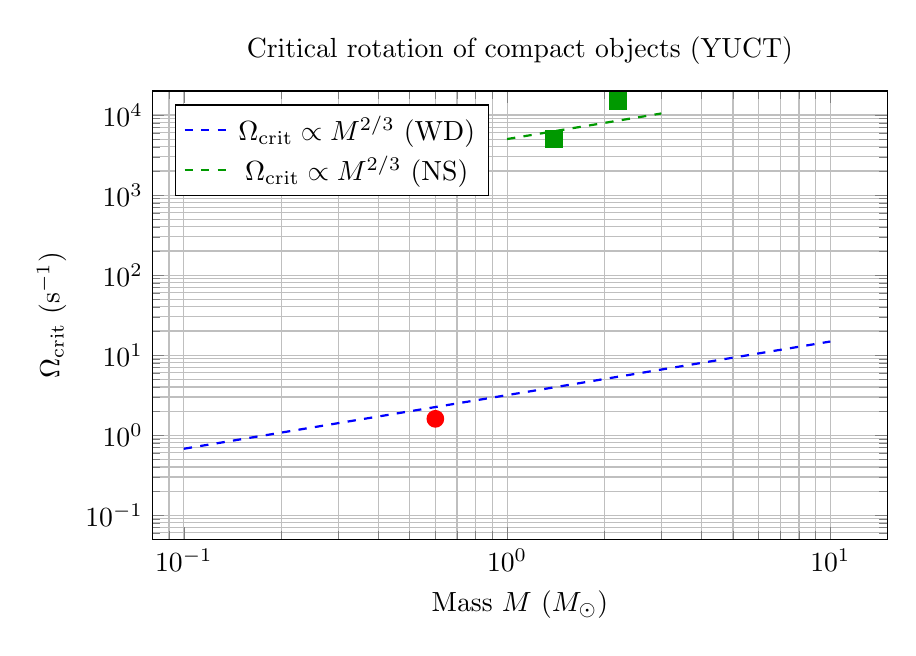
\begin{tikzpicture}
				\begin{loglogaxis}[
					xlabel={Mass \(M\) (\(M_\odot\))}, ylabel={\(\Omega_{\mathrm{crit}}\) (s\(^{-1}\))},
					grid=both, width=0.9\textwidth, height=0.6\textwidth,
					legend pos=north west, title={Critical rotation of compact objects (YUCT)},
					xmin=0.08, xmax=15, ymin=5e-2, ymax=2e4,
					]
					\addplot[domain=0.1:10, samples=2, thick, blue, dashed] {10^(0.67*log10(x)+0.5)};
					\addlegendentry{\(\Omega_{\mathrm{crit}}\propto M^{2/3}\) (WD)};
					\addplot[domain=1:3, samples=2, thick, green!60!black, dashed] {10^(0.67*log10(x)+3.7)};
					\addlegendentry{\(\Omega_{\mathrm{crit}}\propto M^{2/3}\) (NS)};
					\addplot[only marks, mark=*, mark size=3pt, red] coordinates {(0.6,1.6)};
					\addplot[only marks, mark=square*, mark size=3pt, green!60!black] coordinates {(1.4,5000) (2.2,15000)};
					\addplot[only marks, mark=triangle*, mark size=3pt, orange] coordinates {(0.2,3e-5)};
				\end{loglogaxis}
			\end{tikzpicture}
			\caption{السرعة الزاوية الحرجة مقابل الكتلة (YUCT). تؤكد الميول \(\beta=2/3\).}
			\label{fig:omega-mass}
		\end{figure}
	\end{otherlanguage}
	
	\section{تنبؤات قابلة للتكذيب}
	
	\begin{enumerate}
		\item \textbf{بقايا الثقوب السوداء البدائية:} \(f_{\mathrm{relic}} \approx 0.05\) من المادة المظلمة. تُدحض إذا كانت \(f_{\mathrm{relic}}>0.2\) أو \(<0.01\) عند مستوى ثقة 95\%.
		\item \textbf{معاملات التضخم:} \(n_s = 0.965\pm0.005\)، \(r\approx 0.07\). تُستبعد إذا كان \(r<0.01\) أو \(n_s\) خارج \(0.960\pm0.010\).
		\item \textbf{اللا غاوسية:} \(f_{\mathrm{NL}}^{\mathrm{local}} \approx 1.12\). تُكذَّب إذا قيست \(<0.5\) أو \(>1.8\) عند \(>3\sigma\).
		\item \textbf{انحراف مخبري عن \(E=mc^2\):} \(\Delta E/E \sim \kappa_c\alpha K_{\mathrm{eff}}^{-\beta}\). نتيجة صفرية عند حساسية \(10^{-18}\) ستشكل تحدياً لـ YUCT.
		\item \textbf{دورة الدوران الكوني:} \(T_{\mathrm{rot}} \approx 2.3\times10^{14}\) سنة. ستعمل المسوحات المستقبلية (Euclid, SKA) على تنقيح \(\omega\).
	\end{enumerate}
	
	\section{خلاصة}
	
	توحد مسلمات YUCT الكتلة الحرجة لانفجار عظيم موضعي، وقابليات الرصد التضخمية، والدوران الشامل للكون، والتسلسل الهرمي الكامل للكتلة من بذرة بلانك إلى الكون المرصود. جميع التنبؤات كمية وقابلة للتكذيب. لُخِّصت المعادلات الأساسية أعلاه، وكل منها موسومة كعلاقة YUCT. الاشتقاقات المفصلة متوفرة في الملاحق المذكورة.
	
	\section*{توفر البيانات}
	
	الاشتقاقات الكاملة والكود: \url{https://github.com/Alexey-Yakushev-YUCT/YPSDC}
	
	\section*{مراجع لملاحق YUCT}
	\begin{itemize}
		\item الملحق L: قياس الخطأ الكسيري للتنسيق – القانون الشامل \(\beta=2/3\)، \(d_f=11/5\).
		\item الملحق Y: الأسس الرياضية واشتقاق KPZ.
		\item الملحق P: اعتماد الجاذبية على درجة الحرارة.
		\item الملحق M: التضخم كانقال طور تنسيقي.
		\item الملحق \(\Omega\): الدوران الشامل للكون.
		\item الملحق B: بروتوكول YPSDC.
	\end{itemize}
	
\end{document}